\documentclass{article}


\setlength{\parindent}{1,25cm}

\author{Сыров Александр Викторович}
\usepackage[utf8]{inputenc}
\usepackage[russian]{babel}  
\usepackage{graphicx}
\usepackage{float}
\usepackage{wrapfig}
\usepackage{indentfirst}
\usepackage{amsmath}
\usepackage{biblatex}

\addbibresource{mybib.bib}

\begin{document}
	
\begin{titlepage}
	\begin{center}
		Министерство образования и науки РФ
		ФГАОУ ВО Дальневосточный федеральный университет \flqq ДВФУ\frqq\\
		Школа естественных наук\\
		Кафедра компьютерных систем\\
	\end{center}
	\vspace{5cm}
	\begin{center}
		\LARGE \bf{Выдуманный диплом}
	\end{center}
	\begin{center}\large
		Диплом на соискание степени бакалавра
	\end{center}
	\vspace{3cm}
	\large
	\begin{flushright}
		\textbf{Выполнил:}\\
		студент группы Б8116-09.03.02\\
		Сыров Александр Викторович\\
		\vspace{1cm}
		\textbf{Научный руководитель:}\\
		док. физ.-мат. наук \\
		профессор Петров Пётр Петрович
	\end{flushright}
	\vspace{1cm}
	\begin{center}
		Владивосток 2020
	\end{center}
\end{titlepage}

\section{Инструкция по развертке локальной сети} \label{s1}

Автор данной PDF: Сыров Александр Викторович.

\subsection{Введение} \label{s1:s1}

Таблицы, совершенно неупомянутые в этом разделе, можно найти в \ref{s1:s4}.

Локальная сеть на данный момент является важной составляющей любого предприятия, использующего в своей работе компьютеры. Локальная сеть позволяет упростить многие бизнес-процессы, повысить контроль за качеством работы. Место для елочки снизу \ref{fig:elka_bottom}.


Целью данной работы является написание инструкции по развертыванию локальной сети в типографии. Необходимо исследовать предприятие, на котором будет развертываться локальная сеть, его бизнес-процессы и потоки данных, определить, какое необходимо оборудование и программное обеспечения для успешного развертывания локальной сети.\cite{ellis1990annotated}

Тут будет ссылка на елку, которая сверху \ref{fig:elka_top}.

\subsection{Общее описание} \label{s1:s2}

Типография, для которой требуется развернуть локальная сеть, занимается производством различной типографской продукции. Локальная сеть необходима для организации полного цикла рабочего процесса от заказа клиента до готового изделия.\cite{coplien1992advanced}

Данное предприятие располагается в двух зданиях: офисе и цехе. Офис состоит из 3 кабинетов, предназначенных для части работников типографии. Цех находится на определенном удалении от офиса, более 1 км. Цех состоит из 4 больших комнат с различными станками. \cite{barton1994scientific}

И место для елочки по месту \ref{fig:elka_here}.

\newpage

\subsection{Картинки} \label{s1:s3}

В этом параграфе расположенно несколько картинок.

\begin{figure}[t!]
	\center{
\includegraphics[scale=0.3]{../img/tree.png}}
	\caption{Елка, расположенная сверху}
	\label{fig:elka_top}
\end{figure}

Так же использую его для ссылок на формулы. Согласно формуле \ref{equ_1} и формуле \ref{equ_2} все будет хорошо, а по формуле \ref{equ_3} все вдвое лучше.

\begin{figure}[h!]
	\center{
\includegraphics[scale=0.3]{../img/tree.png}}
	\caption{Елка по месту}
	\label{fig:elka_here}
\end{figure}

\begin{figure}[b!]
	\center{
\includegraphics[scale=0.3]{../img/tree.png}}
	\caption{Елка, расположенная снизу}
	\label{fig:elka_bottom}
\end{figure}

\newpage

\subsection{Формулы} \label{s1:s4}

Кроме формул, изложенных ниже, стоит так же упомянуть таблицы \ref{table:table_1} и \ref{table:table_2}.

\begin{equation} \label{eu_eqn}
    e^{\pi i} + 1 = 0
\end{equation}

\begin{equation} \label{equ_1}
	\begin{matrix}
		a + b = \\
		& = c + d
	\end{matrix}
\end{equation}

\begin{equation} \label{equ_2}
	\begin{matrix}
		a + b = \\
		& = c + d * 2
	\end{matrix}
\end{equation}

\begin{align} \label{equ_3}
	a + b & = \nonumber \\
	& = c + d
\end{align}

Замечательное равенство \ref{eu_eqn} известно также как тождество Эйлера.

\newpage

\subsection{Таблицы} \label{s1:s5}

Данный раздел содержит две таблицы. Есть несколько причин создания этих таблиц:

\begin{itemize}
	\itemНадо;
	\itemОчень надо;
	\itemСовсем надо.
\end{itemize}

И еще один списочек, но на этом раз нумерованный:

\begin{enumerate}
	\item Списки классно!
	\item Списки очень классно!
	\item И тут их можно стилизовать!
\end{enumerate}

А так же стоит упомянуть, что картинки расположены в разделе \ref{s1:s3}.

\begin{table}[t]
	\caption{Первые искусственные спутники Земли}
	\centering
	\begin{tabular}{ | l | l | l |}
	\hline
	ИСЗ & Дата запуска & Масса, кг      \\ \hline
	Спутник-1 & 4 октября 1957 & 83.6   \\ \hline
	Спутник-2 & 3 ноября 1957 & 508.3   \\ \hline
	Эксплорер-1 & 1 февраля 1958 & 21.5 \\
	\hline
	\end{tabular}
	\label{table:table_1}
\end{table}

\begin{table}[h]
	\caption{Просто цифры}
	\centering
	\begin{tabular}{ | l | l | l |}
	\hline
	1 & 2 & 3      \\ \hline
	3 & 4 & 5   \\ \hline
	6 & 7 & 8   \\
	\hline
	\end{tabular}
	\label{table:table_2}
\end{table}

\subsection{Использование Gnuplot} \label{s1:s6}

Данные были взяты с сайта сбора статистики по YouTube-каналам. С помощью GNU Plot исходные данные были выведены на график, и было замечено, что график роста подписчиков практически линейный. В качесте функции аппроксимации была взята функция $ y = 447 + 1.9 * x $, где $x$ - номер дня на графике, начиная с нуля.

Для генерации конечного графика был написан и использован следующий скрипт:

\begin{verbatim}
set terminal png
set output 'plot.png'

set title "Количество подписчиков случайного YouTube-канала"
set xlabel "Дата"
set ylabel "Количество подписчиков(тыс.)"

set xdata time
set timefmt "%Y-%m-%d"
plot "data.tsv" using 1:2 title "Данные", "data.tsv" using 1:3 title "аппроксимация" with lines
\end{verbatim}

\begin{figure}[h!]
	\center{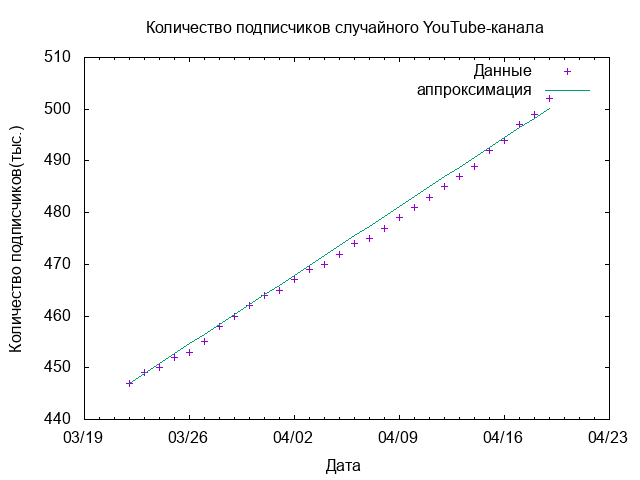
\includegraphics[scale=0.7]{../plots/plot.png}}
	\caption{График роста подписчиков случайного YouTube-канала}
	\label{fig:gnuplot}
\end{figure}

\newpage

\tableofcontents
\newpage
\printbibliography
\end{document}